\chapter{Experiment}
\label{ch:experiment}

In dit hoofdstuk worden de resultaten besproken van het experiment tussen Vuforia en ARCore. De eerste sectie van dit hoofdstuk gaat over hoe goed beide frameworks de vijftien afbeeldingen hebben herkent. De achtereenvolgende hoofdstukken hebben te maken met de analyse van de data uit het experiment. Tot slot is er een conclusie waarin één van de frameworks bekroond is als winnaar.

\section{Afbeeldingsherkenning}
Bij de vijf initiële experimenten heeft ARCore alle afbeeldingen herkent terwijl Vuforia één afbeelding niet kon herkennen namelijk George3 (te vinden op de \href{https://github.com/MatthiasDeFre/bachelorproef-hogent-2019}{Github repository van deze studie \autocite{GITHUBMDF}}). Vuforia herkende de afbeelding niet door de lage verlichting die aanwezig was. Wanneer de verlichting op de afbeelding verhoogde herkende Vuforia de afbeelding direct (zie figuur \ref{fig:vuforiaDarkImage}.

\begin{figure}
    \includegraphics[width=\linewidth]{vuforiaDarkImage.png}
    \caption{Vuforia: Het herkennen van een afbeelding gaat niet als er te weinig belichting is}
    \label{fig:vuforiaDarkImage}
\end{figure}


Het interessante aan dit deel van het experiment is dat beide frameworks afbeeldingen met een lage score makkelijk konden herkennen. Vuforia had bijvoorbeeld geen moeite met het herkennen van afbeelding George1 die maar een score heeft van één ster. ARCore kon afbeelding George4 (score 0) en augmentedImageBad1 (score 5) ook zonder veel moeite herkennen.

ARCore scoort dus bij dit onderdeel iets beter door het herkennen van afbeeldingen in donkere ruimtes.

\section{FPS}\label{sec:fps}

Uit de data van beide frameworks blijkt het dat Vuforia maximum 60 FPS kan halen terwijl ARCore maar een maximum behaalt van 30 FPS. Het halen van een 60 FPS is redelijk onbelangrijk omdat vele Android Smartphones (vooral de iets oudere) nog geen 60 FPS camera ondersteunen. Het belangrijkste is een constant framerate behouden zonder veel grote FPS drops.

Om na te kijken of het framework een constant framerate kan behouden wordt de standaardafwijking gebruikt. Een kleine standaardafwijking wijst er namelijk op dat de datapunten weinig afwijken van het gemiddelde.

\begin{itemize}
    \item Vuforia: 1,60
    \item ARCore: 1.03
\end{itemize}

Beide frameworks hebben een kleine standaardafwijking wat er op wijst dat hun framerate redelijk (maar niet honderd procent) constant is. 

Een standaardafwijking groter dan nul wijst erop dat data niet constant is. Bij beide frameworks zijn er dus FPS drops aanwezig.

De grote van de FPS drops hebben een grotere impact op de ervaring dan de frequentie van de drops. Kleine drops van één tot twee frames hebben geen impact op de ervaring voor gebruiker omdat ze niet zichtbaar zijn. Daarom analyseert deze studie alleen maar de FPS drops die groter zijn dan tien frames.

\begin{itemize}
    \item Vuforia: 5
    \item ARCore: 3
\end{itemize}

\subsection{Analyse FPS Drops: Vuforia}

De oorsprong van de FPS drops bij Vuforia is makkelijk te achterhalen door naar het tijdstip te kijken wanneer ze voorkomen (zie tabel \ref{tbl:vuforiadrop}). In deze tabel is duidelijk te zien dat de drops altijd voorkomen bij het opstarten van de applicatie.

\begin{table}
    \centering
    \begin{tabular}{llllll}\toprule
        & \textit{Drop 1}   & \textit{Drop 2}   & \textit{Drop 3}   & \textit{Drop 4}   & \textit{Drop 5}   \\ \midrule
        Experiment         & 1        & 2        & 3        & 4        & 5        \\
        Tijdstip in seconden          & 1.003758 & 1.015506 & 1.013395 & 1.012443 & 1.012150 \\
        Frames per seconde & 33       & 34       & 32       & 34       & 34      \\ \bottomrule
    \end{tabular}
    \caption{Vuforia: grote FPS drops komen eenmalig in het begin voor bij elk experiment}\label{tbl:vuforiadrop}
\end{table}

Op figuur \ref{fig:vuforiaTimeDrop} is te zien dat de framerate voor het verdere verloop van de applicatie stabiel blijft met hier en daar een kleine FPS (minder dan 10 frames) drop.

\begin{figure}
    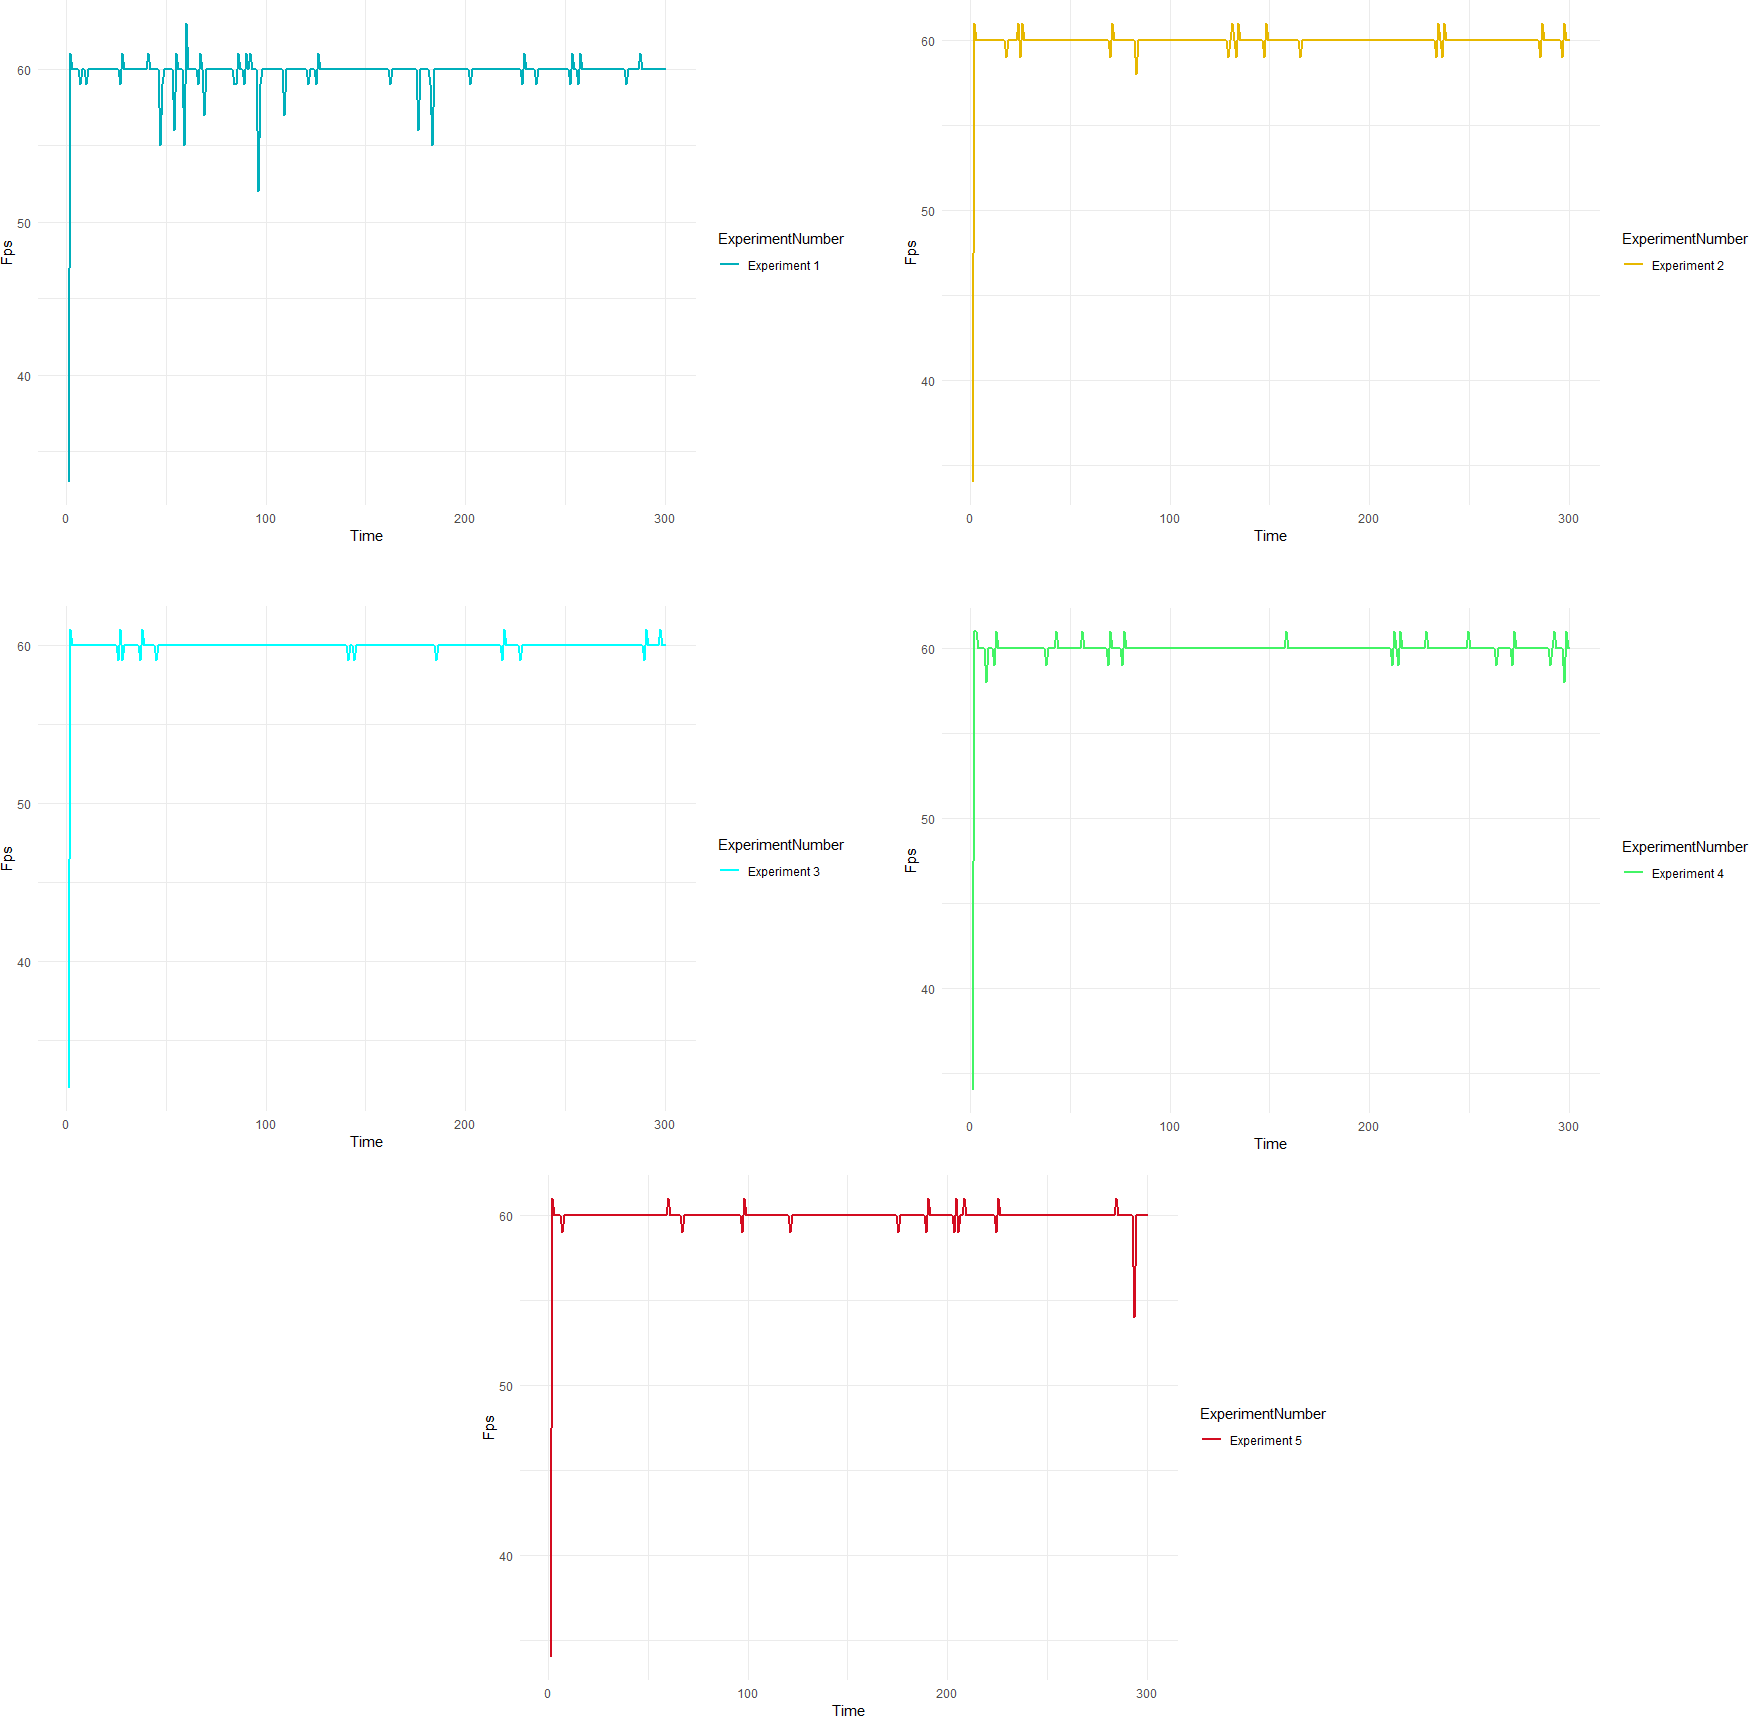
\includegraphics[width=\linewidth]{vuforiaAllExp.png}
    \caption{Vuforia: verloop van de FPS bij alle experimenten (1 tot 5, van links naar rechts en boven naar onder)}
    \label{fig:vuforiaTimeDrop}
\end{figure}

\subsection{Analyse FPS Drops: ARCore}
Hoewel ARCore minder drops heeft dan Vuforia zijn ze wel veel groter (zie tabel \ref{tbl:arcoredrop}) in secties \ref{sec:memory} en \ref{sec:gameobjects} worden de oorzaken van deze drops verder besproken. Op figuur \ref{fig:arcoreTimeDrop} is te zien dat net zoals bij Vuforia de FPS bij alle experimenten redelijk consistent blijft doorheen de applicatie. Het grote verschil met Vuforia is dat de kleinere drops hoofdzakelijk geconcentreerd zijn in het begin (eerste 50 seconden) in plaats van verspreid te doorheen de looptijd van de applicatie. 

\begin{table}
    \centering
    \begin{tabular}{llll} \toprule
        & \textit{Drop 1}    & \textit{Drop 2}   & \textit{Drop 3}    \\ \midrule
        Experiment         & 2         & 4        & 4         \\
        Tijdstip in seconden          & 218.63180 & 85.33646 & 250.73920 \\
        Frames per seconde & 8         & 7        & 10       \\ \bottomrule
    \end{tabular}
    \caption{ARCore: grote FPS drops komen inconsistent voor bij de verschillende experimenten }\label{tbl:arcoredrop}
\end{table}

\begin{figure}
    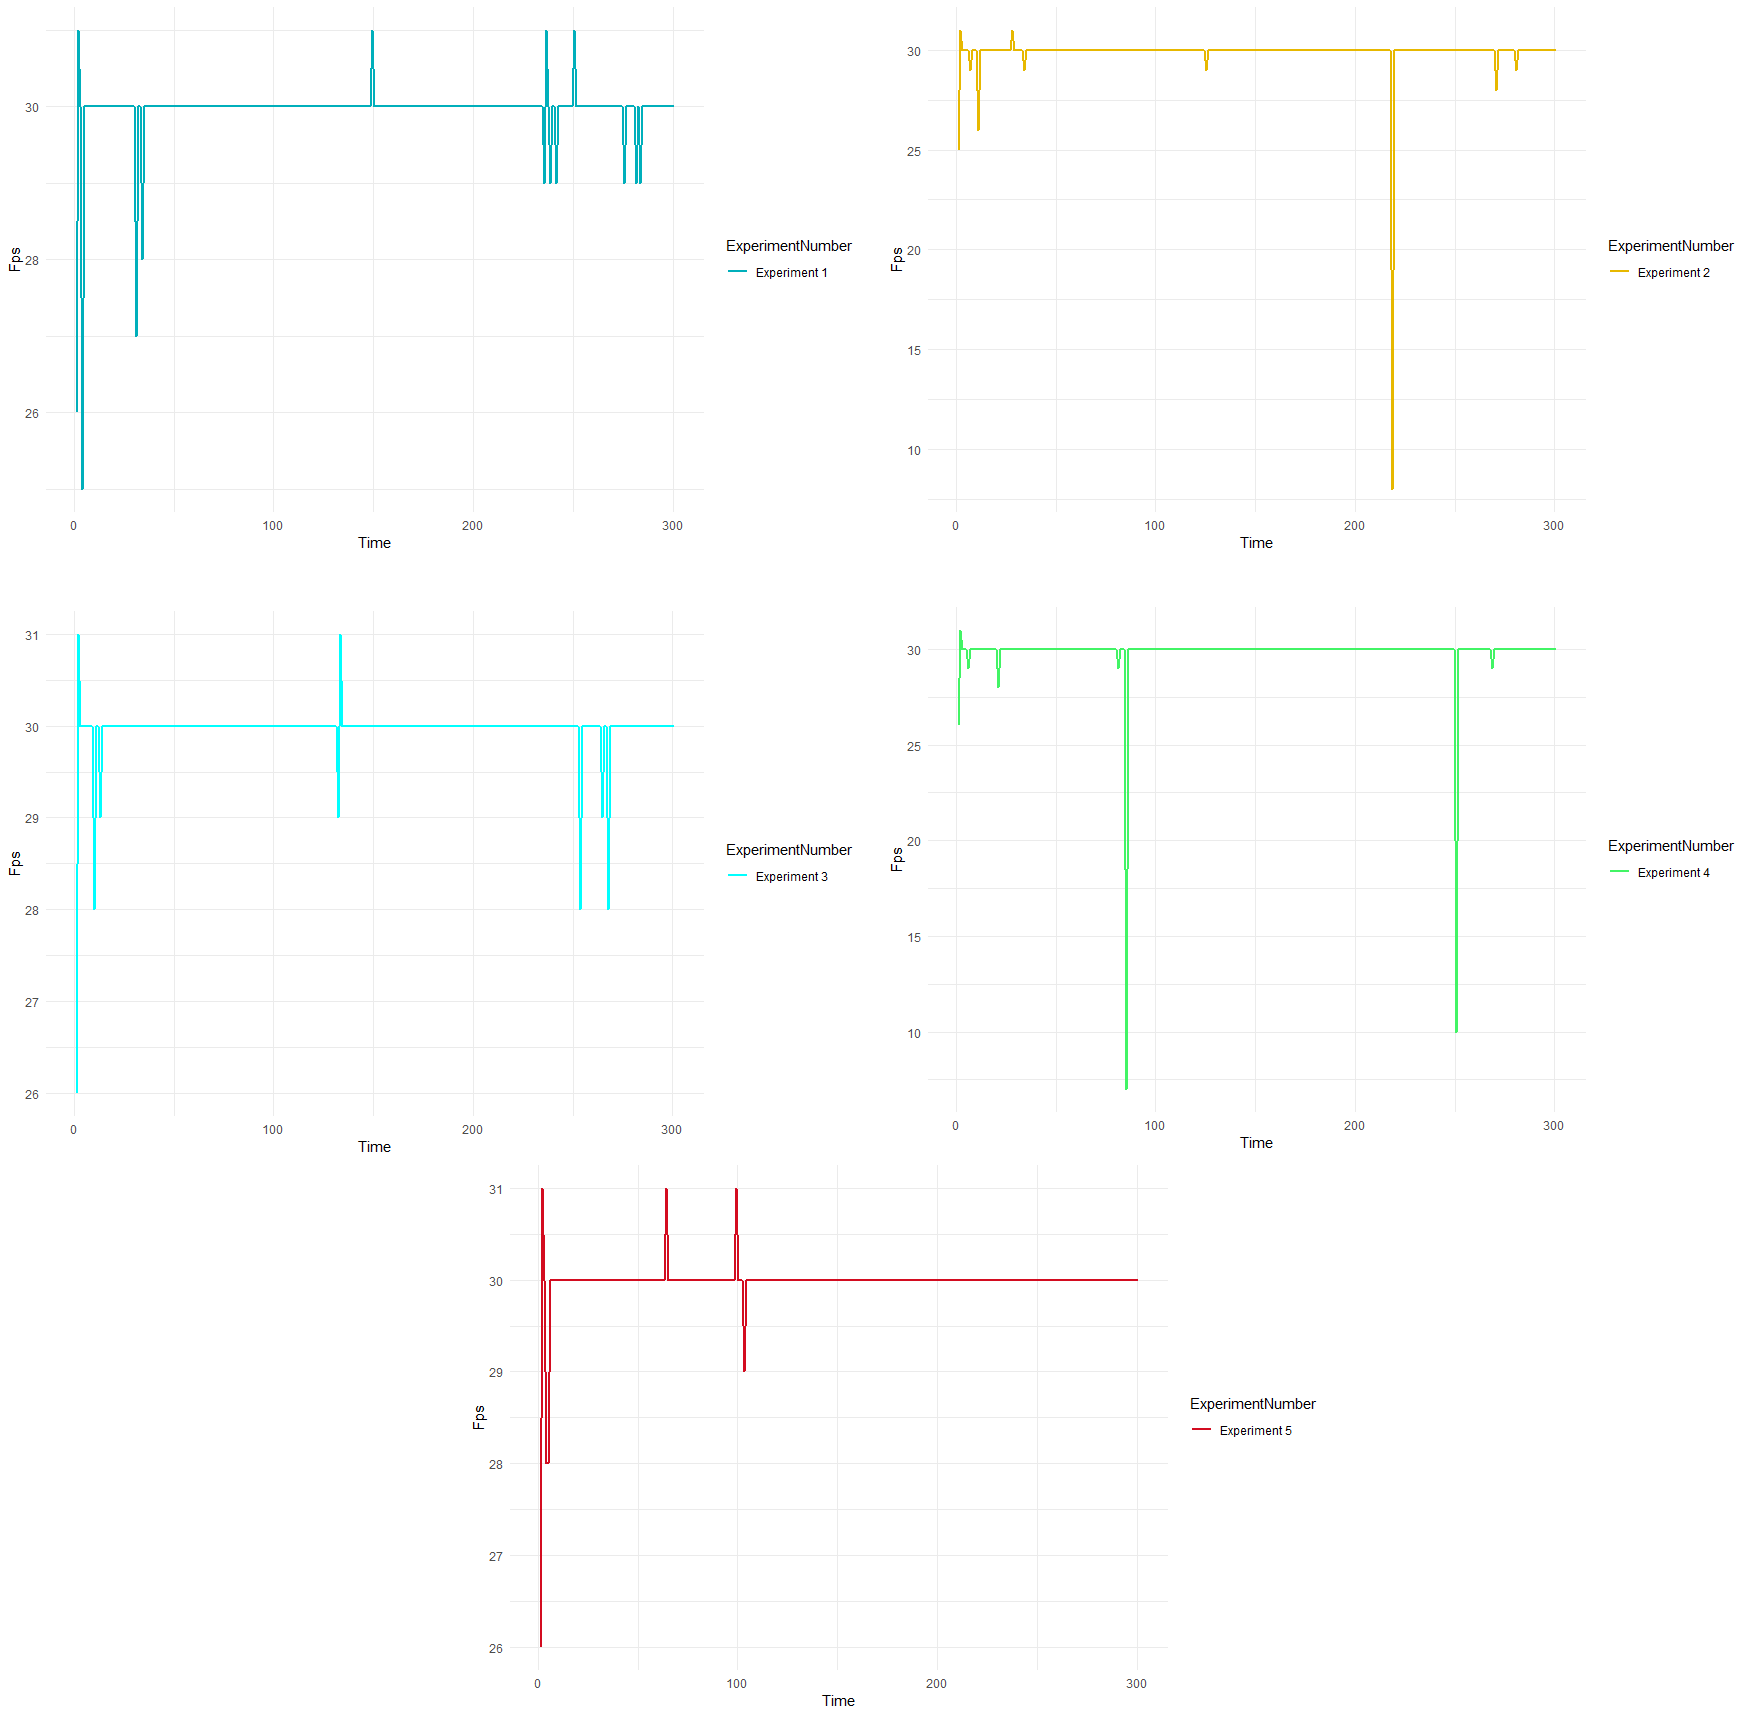
\includegraphics[width=\linewidth]{arcoreAllExp.png}
    \caption{ARCore: verloop van de FPS bij alle experimenten (1 tot 5, van links naar rechts en boven naar onder)}
    \label{fig:arcoreTimeDrop}
\end{figure}

\section{RAM}\label{sec:memory}
Door de gemiddelden en standaardafwijkingen van het gereserveerde en geallorceerde RAM van beide frameworks te berekenen is het duidelijk dat de ARCore applicatie gemiddeld 4MB minder RAM verbruikt dan Vuforia. Dit is ook makkelijk te bewijzen door aan beide datasets een kolom toe te voegen waarin staat tot welk framework ze behoren en deze datasets samen te voegen. Op deze nieuwe dataset is een t-test uitgevoerd die als resultaat een p-waarde van 1 had wat erop wijst dat er een sterk verband is tussen het gekozen framework en het verbruikte RAM.

Het RAM-verbruik van Vuforia fluctueert ook veel meer dan ARCore, een standaardafwijking van 4.5MB tegenover 0.06MB. Dit is ook te bewijzen door een t-test uit te voeren op een nieuwe kolom die het vorige RAM - het huidige RAM bevat. Het resultaat van deze test was een p-waarde van 0.7419 wat aantoont dat het RAM-verbruik van ARCore inderdaad stabieler is.

Wanneer het gereserveerde RAM stijgt is het ook logisch dat gealloceerde RAM stijgt. Een applicatie gaat niet meer RAM reserveren tenzij deze meer RAM nodig heeft. Dit is bewezen door het correlatiecoëfficiënt van gereserveerd tegenover gealloceerd RAM en het correlatiecoëfficiënt van de stijging in gereserveerd RAM tegenover de stijging in gealloceerd RAM te berekenen. In tabel \ref{tbl:ramcor} is te zien dat bij beide frameworks hier een volstrekt verband is.

\begin{table}
    \centering
    \begin{tabular}{lll} \toprule
       \textit{Frameworks} &  \textit{Gereserveerd vs gealloceerd} &  \textit{Stijging gereserveerd   vs stijging gealloceerd} \\ \midrule
        Vuforia & 0.9987308                          & 0.9496204                                            \\ 
        ARCore  & 0.9981332                          & 0.9999941                                           \\ \bottomrule
    \end{tabular}
 \caption{De correlatiecoëfficiënten gereserveerd en gealloceerd RAM (en hun stijgingen) tonen een duidelijk verband}\label{tbl:ramcor}
\end{table}

\subsection{Correlatie RAM en FPS}
Zoals er eerder vermeld in sectie \ref{sec:fps} kampen beide frameworks met FPS drops. Om deze FPS drops te verklaren is er onderzoek gedaan of er een verband is tussen stijgingen in RAM-verbruik en FPS.

Uit de tabellen \ref{tbl:ramfps} en \ref{tbl:ramdropfps} is het duidelijk dat er bij Vuforia een verband aanwezig is tussen stijgingen in gereserveerd en gealloceerd RAM en FPS drops. Tussen deze stijgingen en FPS is er een negatief verband aanwezig wat erop wijst dat de FPS zal dalen wanneer er een stijging zal plaatsenvinden. Dit wordt ook nog eens bevestigd in \ref{tbl:ramdropfps} waarbij er een positief verband aanwezig is wat wijst op een stijging in het aantal gedropte frames wanneer het RAM stijgt. Bij ARCore is er alleen bij de FPS drops een verband aanwezig. Dit is te verklaren door de grote FPS drops die Vuforia ervaart bij het opstarten van de applicatie.
\begin{table}
    \centering
    \begin{tabular}{lllll}\toprule
       \textit{Frameworks} & \textit{Reserveerd} & \textit{Stijging reserveerd} & \textit{Alloceerd}  & \textit{Stijging alloceerd} \\ \midrule
        Vuforia & 0.01598619 & -0.9604763          & 0.01714372 & -0.9107168         \\ 
        ARCore  & 0.04140291 & -0.2194807          & 0.04099924 & -0.2321268        \\ \bottomrule
    \end{tabular}
\caption{Correlatie tussen RAM en FPS, een stijging van gereserveerd of gealloceerd RAM doet de FPS dalen bij Vuforia, ARCore heeft hierbij een zwakker negatief verband. Het totaal aantal RAM heeft geen verband met de FPS}\label{tbl:ramfps}
\end{table}

\begin{table}
    \centering
    \begin{tabular}{lllll}\toprule
        \textit{Frameworks} & \textit{Reserveerd}   & \textit{Stijging reserveerd} & \textit{Alloceerd}   & \textit{Stijging alloceerd} \\ \midrule
        Vuforia & -0.005773322 & 0.7445151           & -0.00729054 & 0.6988763          \\
        ARCore  & -0.1287283   & 0.7155269           & -0.1315688  & 0.7157725   \\    \bottomrule 
    \end{tabular}
\caption{Correlatie tussen RAM en FPS drops, een stijging van gereserveerd of gealloceerd RAM vermeerdert de FPS drop bij Vuforia en ARCore, totaal aantal RAM heeft geen verband met de grootte}\label{tbl:ramdropfps}
\end{table}

\section{GameObjects}\label{sec:gameobjects}
Ook het aantal gameobjects kon invloed hebben op FPS drops. Het interessante verschil tussen Vuforia en ARCore is de standaard methode waarop ze de virtuele objecten onthouden. Omdat bij Vuforia het object een kind is van het image target is deze sowieso aanwezig zelfs wanneer de afbeelding nog niet herkent is. Het aantal objecten is bij Vuforia constant, dit is makkelijk na te gaan door de standaardafwijking te berekenen die nul uitkomt wat wijst op geen afwijkingen. Om te objecten niet constant in te wereld te moeten tonen ze Vuforia hun renderer uit wanneer ze niet meer zichtbaar zijn. Het aantal zichtbare objecten (deze waarvan de renderer aanstaat) heeft helemaal geen (-0.006362351) invloed op het RAM.

ARCore werkt op een volledige andere manier voor het bijhouden van de objecten. In de code van het standaard script staat er dat wanneer een nieuwe afbeelding wordt herkent er hiervoor een nieuw gameobject nodig is. Bij het verliezen van de tracking vernietigt het script dit object. Met deze manier van werken is het aantal actieve objecten dus niet constant. Op de grafiek van figuur \ref{fig:arcoreObjectCount} is er te zien dat de oude objecten niet verdwijnen uit het geheugen. Door het variabel aantal objecten is het mogelijk om de correlatie tussen aantal objecten en RAM-verbruik na te gaan. Er is inderdaad een positief (0.6887693) verband aanwezig. Om na te gaan of dit correct is, is het verband tussen de stijgingen in aantal objecten en stijgingen in RAM gecontroleerd wat ook een positief verband aantoont (0.6253159). 

\begin{figure}
    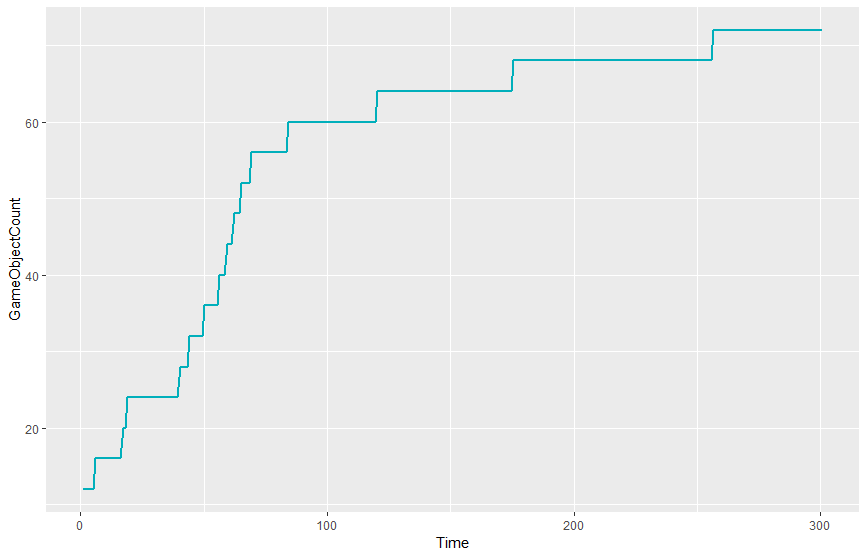
\includegraphics[width=\linewidth]{arcoreObjectCount.png}
    \caption{Verloop van het aantal objecten van ARCore bij experiment 4}
    \label{fig:arcoreObjectCount}
\end{figure}

Het is wel belangrijk dat deze analyse is uitgevoerd op de standaard scripts en dat door aanpassingen aan deze scripts de resultaten positief of negatief zullen veranderen. De methode van Vuforia werkt ook, mits kleine aanpassingen, bij ARCore en vice-versa wat voor andere resultaten zal zorgen.

\section{Constatering Voortreffelijkste Framework}
De analyse van de FPS wijst erop dat Vuforia wel meer future proof is door nu al 60 FPS te ondersteunen tewijl ARCore maar maximum 30 FPS aankan. 
Wel is het duidelijk dat de FPS van ARCore wel iets stabieler is dan de FPS van Vuforia zoals te zien op de grafieken in figuren \ref{fig:vuforiaTimeDrop} en \ref{fig:arcoreTimeDrop}. 
Ook bij RAM-verbruik en RAM-stijgingen zien we dat ARCore beter scoort door alleen de objecten in te laden die momenteel herkent zijn. 
Dit verband is belangrijk omdat, zoals bewezen, stijgingen in RAM een invloed hebben op de groote van de FPS drops.
Een kleine stijging of een klein aantal stijgingen is hierbij dus belangrijk.

Voor deze redenen is ARCore dus de winnaar van het experiment en is hiervoor een prototype gemaakt dat te zien is in hoofdstuk \ref{ch:prototype}.
